%%%%%%%%%%%%%%%%%%%%%%%%%%%%%%%%%%%%%%%%%%%%%%%%%%%%%%%%%%%%%%%%%%%%%%%%%%%%%%%%%%%%%%%%
\chapter[Quantum Order and Projective Symmetry Groups]{Quantum Order and\linebreak Projective Symmetry Groups}
\label{chapter:ProjectiveSymmetryGroup}
%%%%%%%%%%%%%%%%%%%%%%%%%%%%%%%%%%%%%%%%%%%%%%%%%%%%%%%%%%%%%%%%%%%%%%%%%%%%%%%%%%%%%%%%
%
%
On the topic of approaching new problems in physics, P.~W. Anderson wrote in his 1984 textbook \textit{Basic notions of condensed matter physics}~\cite{Anderson1984},
%
\begin{quote}
	"the two most important principles of condensed matter physics~\ldots~are, first, broken symmetry, which tells us what the order parameter is and what symmetry it breaks are the most vital questions; and, second, the continuity principle, which tells us to search for the right simple problem when confronted with a complicated one."
\end{quote}
%
In the former case, he is referring to Landau's theory of phase transitions~\cite{LandauNature1936,LandauZETF1937,GinzburgZETF1950}.
In regards to the latter, he goes on to use Landau's Fermi liquid theory~\cite{LandauZETF1956,LandauZETF1957,LandauZETF1958} to illustrate the power of the principle of adiabatic continuity.

Landau's theory of phase transitions makes the observation that, given a Hamiltonian $\op{H}$ along with a symmetry group $G$ which preserves it, although the Hamiltonian may possess a given symmetry, the dynamics of the system singles out a ground state which breaks that symmetry.
This process goes by the name of \textit{spontaneous symmetry breaking}.
According to Landau's theory, different phases of matter can be distinguished by their symmetries.
Thus, a given Hamiltonian in different parameter or temperature regimes may give rise to different phases of matter by virtue of the mechanism of spontaneous symmetry breaking.

Landau's theory, furthermore, allows for the definition of a local order parameter which signals the spontaneous breaking of a symmetry and, thus, the onset of order in the system.
A ground state of the system is seen not to be invariant under $G$ if there exists an order parameter $\op{O}$ and one $g \in G$ such that $g \op{O} \neq \op{O}$ and $\psi_{\op{O}} \equiv \avg{\op{O}} \neq 0$.
Any specific ground state is characterized by a maximal subgroup $H$ which still preserves it, \ie,
%
\begin{align}
	\psi_{h \op{O}} &= \psi_{\op{O}} \qquad \forall h \in H \nonumber\\
	\psi_{g \op{O}} &\neq \psi_{\op{O}} \qquad \forall g \in G/H.
\end{align}
%
Having identified the order parameter, one may write down an effective free energy functional for the system in terms of $\psi_{\op{O}}$ in the vicinity of the phase transition, yielding a mean-field description of the transition from the disordered phase to the ordered phase. 
The combination of Landau's theory with the ideas of Wilson's renormalization group~\cite{WilsonPRB1971I,WilsonPRB1971II,WilsonPRL1972,WilsonRMP1975} allowed for the definition of \textit{universality classes}, unifying phase transitions in seemingly disparate physical systems into equivalence classes defined by their universal critical behavior.
Additionally, Nambu and Goldstone~\cite{NambuPRL1960,GoldstoneINC1961} showed that a generic spontaneously broken continuous symmetry implies the existence of massless scalar bosons corresponding to long-wavelength excitations of the order parameter.
This synthesis of ideas has been wildly successful and it was long thought to provide a complete understanding of the different phases of matter.

Landau's Fermi liquid theory has been similarly fruitful, providing a\linebreak phenomenological description of many strongly interacting fermion systems such as (normal) liquid $^3$He and normal metals~\cite{SilinJETP1958,SilinJETP1959} in terms of \textit{nearly free}\linebreak \textit{fermions}~\cite{Leggett2006}.
Landau argued that, in the absence of an electronic phase transition, the ground state of the non-interacting Fermi gas would be adiabatically transformed into the ground state of the interacting system as the interaction strength was slowly increased.
Furthermore, he assumed that each excited state of the ideal Fermi gas is likewise adiabatically transformed into a corresponding excited state of the interacting Fermi liquid, \ie, there is a one-to-one correspondence between the particle and hole excitations of the Fermi gas and the so-called \textit{quasiparticle} and \textit{quasihole} excitations of the Fermi liquid which carry the same spin, charge and momentum as the excitations in the non-interacting system, but with a different \textit{effective mass}.\footnote{For simplicity, a momentum- and spin-conserving potential is assumed.}

A consistent application of Fermi liquid theory must also include interactions between quasiparticles (quasiholes) at lowest order and, thus, scattering between quasiparticles, leading to a finite quasiparticle lifetime.
Such a finite lifetime would seem to spoil the above arguments which depend on the adiabatic evolution of free fermions into quasiparticles, however, for excitations sufficiently close to the Fermi surface (as one would expect for low temperatures), the quasiparticle lifetimes become sufficiently long to justify the established one-to-one correspondence between quasiparticle excitations of the Fermi liquid and excitations of the Fermi gas.
This \textit{nearly free} quasiparticle picture results in certain equilibrium properties of the Fermi liquid such as specific heat, static compressibility, spin- and charge-susceptibilities being qualitatively unchanged from those of the ideal Fermi gas at low temperatures, with prefactors simply being renormalized by replacing the bare mass with the effective mass and/or by effects of quasiparticle scattering~\cite{Pines1966,Coleman2015}.
Besides just possessing renormalized properties of a Fermi gas, the Fermi liquid also has entirely new characteristics such as \textit{zero sound} -- supersonic density oscillations in the Fermi liquid resulting from interactions between the quasiparticles~\cite{KeenPL1963,AbelPRL1966,MerminPR1967}.

Landau already understood that the Fermi liquid theory is always potentially unstable to superconductivity as it implies the presence of a phase transition.
By the late 1960's it became clear that a Fermi liquid is generically unstable in one-dimension, giving rise instead to a separation of spin and charge degrees of freedom in what is now known as a Luttinger liquid~\cite{LuttingerJMP1963,HaldaneJoPC1981}.
Eventually, the Fermi liquid theory was given a more rigorous footing in terms of the renormalization group theory, (re)establishing its inapplicability in one-dimension, as well its instability to superconductivity, or to the formation of charge- or spin-density wave orders for nested Fermi surfaces in two- and three-dimensions~\cite{BenfattoPRB1990,ShankarRMP1994}.
However, the renormalization group approach also showed that the Fermi liquid is not \textit{generically} unstable in two- and three-dimensions as it is in 1D, implying a wide range of applicability.

The overwhelming effectiveness of these two theories in describing the physics of many-body systems lead to a feeling that there were no new important concepts to find and that the only thing left to do was apply Landau's theories to different kinds of systems~\cite{Wen2004}.
However, the discovery of the fractional quantum Hall effect by Tsui, St\"ormer and Gossard~\cite{TsuiPRL1982} and its phenomenological description by Laughlin~\cite{LaughlinPRL1983} as a new type of quantum liquid lead to the realization that Landau's theories could not be used to describe \textit{all} states of matter~\cite{WenPRB1989,WenPRB1990}.
Different fractional quantum Hall (FQH) states possess the same symmetry and, thus, cannot be characterized by the paradigm of symmetry breaking.

The concept of \textit{topological order} was introduced~\cite{WenJMPB1990,WenAiP1995} to characterize these states for which no physical, local order parameter could be defined and which host fractionalized collective excitations possessing quantum numbers distinct from those of the electrons from which they are formed.
The theory of topological order proposed to characterize different FQH states by the differing topology of their respective wave functions.
Such a classification is successful for a class of FQH states called Abelian FQH states, \ie, those states for which the low-energy excitations obey Abelian statistics~\cite{BlokPRB1990a,BlokPRB1990b,ReadPRL1990,FroehlichNPB1991,FroehlichRMP1993}.
The non-trivial topology of the FQH wave functions leads to a robust topological ground state degeneracy which depends only on the genus of the surface on which the theory is defined~\cite{HaldanePRL1983,HaldanePRB1985,WenPRB1990}.
Furthermore, the non-trivial topology of the bulk wave function implies the existence of gapless excitations on the surface of the FQH liquid~\cite{WenIJMP1992}.

While topological order can be used to describe a large class of \textit{gapped} quantum liquids such as the Abelian FQH states, the broader designation of \textit{quantum order} can be applied to a broader class of systems (including \textit{gapless} quantum liquids), of which the topologically ordered systems form a subclass.
Quantum order aims to describe the universality classes of quantum ground states as opposed to the universality classes of classical statistical states described by Landau's theory~\cite{WenPRB2002,WenPLA2002}.
There is currently no complete theory to describe all possible quantum orders, however, a large class of quantum orders can be described by an object called a \textit{projective symmetry group} (PSG).
Whereas Landau's theory distinguished classical phases by their symmetries and determined the structure of low-energy excitations without needing to know the details of a system~\cite{NambuPRL1960,GoldstoneINC1961}, the PSG allows for the classification of different \textit{quantum} phases which have the same symmetry, while similarly determining the structure of low-energy excitations without the need to know the details of a system.
In remarkable contrast to symmetry-breaking orders which generate and protect gapless, scalar Nambu-Goldstone bosons, quantum orders can generate and protect gapless gauge bosons and gapless fermions, even in pure local bosonic models~\cite{Wen2004}.

The remainder of this chapter is structured as follows.
The basic ideas behind the PSG are introduced in Section~\ref{section:chapter04_OverviewOfTheProjectiveSymmetryGroup} as well as the ideas behind its use in classifying quantum ground states in the context of quantum spin liquids.
These concepts are developed in greater detail in Sections~\ref{section:chapter04_ProjectiveConstructionOfQuantumSpinLiquids}--\ref{section:chapter04_TheProjectiveSymmetryGroup}.
In Section~\ref{section:chapter04_ApplicationToTheKitaevHoneycombModel}, these concepts are applied to the Kitaev honeycomb model discussed in Chapter~\ref{chapter:KitaevHoneycombModel}.
Finally, Section~\ref{section:chapter04_Summary} provides a brief summary.


%
%%%%%%%%%%%%%%%%%%%%%%%%%%%%%%%%%%%%%%%%%%%%%%%%%%%%%%%%%%%%%%%%%%%%%%%%%%%%%%%%%%%%%%%%
\section{Overview of the projective symmetry group}
\label{section:chapter04_OverviewOfTheProjectiveSymmetryGroup}
%%%%%%%%%%%%%%%%%%%%%%%%%%%%%%%%%%%%%%%%%%%%%%%%%%%%%%%%%%%%%%%%%%%%%%%%%%%%%%%%%%%%%%%%
%
This section introduces the basic ideas behind the construction of mean-field spin liquids using the projective symmetry group.
The idea is to provide an overview of concepts that will be made more precise in the following sections.

The starting point is a Hamiltonian of quantum spin-1/2 moments on a lattice, \eg,
%
\begin{equation}
	\op{H}_{\rm spin} = \sum_{i,j} J_{ij}~\bsigma_i \cdot \bsigma_j,
\end{equation}
%
where $\bsigma$ is a vector of Pauli matrices.
In a classically ordered phase, a standard mean-field decoupling of the quantum spins may be performed, resulting in a mean-field Hamiltonian, \eg,
%
\begin{equation}
	\op{H}_{\rm mean} = \sum_{\avg{i,j}} J_{ij} (\avg{\bsigma_i} \cdot \bsigma_j + \bsigma_i \cdot \avg{\bsigma_j} - \avg{\bsigma_i} \cdot \avg{\bsigma_j}),
\end{equation}
%
in order to determine the nature of the classical mean-field ground state.
Moreover, the low energy excitations of the system may be studied by including the fluctuations above the mean-field.
However, in a quantum spin liquid ground state, the spins do not order even at zero temperature and, thus, the above spin mean-field decoupling fails due to the vanishing expectation value $\avg{\bsigma_i} = 0$, or, more generally, due to the absence of \textit{any} local order parameter.

A possible solution to this problem came in the form of the slave-particle approach~\cite{BaskaranSSC1987}, whereby the spin degrees of freedom are replaced by fermionic partons via the transformation
%
\begin{equation}
	\bsigma_i = f\dag_{i\alpha} \btau_{\alpha\beta} f_{i\beta},
\end{equation}
%
where $\btau$ is the vector of Pauli matrices acting on the spin indices $\alpha,\beta$ of the fermion operators.
This representation comes with the cost of an enlarged Hilbert space due to the inclusion of the unphysical empty and doubly-occupied fermion states.
The advantage, however, is that a mean-field decoupling of the \textit{fermions} rather than of the spins could be performed, with the additional half-filling constraint
%
\begin{equation}
	f\dag_{i\alpha} f_{i\alpha} = 1
\end{equation}
%
being enforced either by Lagrange multiplier or by a Gutzwiller projection of the mean-field state to the physical subspace.

It was later seen~\cite{AffleckPRB1988,DagottoPRB1988} that the parton approach actually contained a hidden local $SU(2)$ gauge redundancy and that the mean-field Hamiltonian could be framed as a quadratic theory of fermions coupled to an $SU(2)$ gauge field.
In this framework, the inclusion of Lagrange multipliers to enforce the half-filling constraint could be interpreted as the temporal component of the $SU(2)$ gauge field.
Now a fermionic mean-field ground state could be found wherein the gauge field is chosen to be static and the restriction of the fermions to the physical, half-filled subspace could be performed by including temporal fluctuations of the gauge field.

It was realized by Wen~\cite{WenPRB2002} that physical symmetry operations on the spins may need to be paired with a gauge transformation in order to preserve a given mean-field configuration and that the exact nature of how symmetries acted in the gauge sector could be an important way of classifying \textit{different} mean-field spin liquids with the \textit{same} symmetries.
The universality classes deriving from this line of thought go by the name \textit{projective symmetry groups}.
A projective symmetry group $PSG$ of a quantum spin liquid phase with symmetry group $SG$ is defined as
%
\begin{equation}
	SG = PSG/IGG,
\end{equation}
%
where $IGG$ is the set of pure gauge transformations leaving the mean-field \textit{Ansatz} unchanged and is known as the \textit{invariant gauge group} (IGG).
In words, the projective symmetry group is the group of combined symmetry and gauge transformations which leave a given mean-field \textit{Ansatz} unchanged up to unitary gauge equivalence.

This idea allowed for the possibility of classifying mean-field spin liquids which possess all of the same symmetries, but which differ in their projective representations.
Additionally, at low energy, fluctuations of the gauge field away from the mean-field \textit{Ansatz} must respect the invariant gauge group, making the IGG an additional way of coarsely classifying different types of mean-field \textit{Ans\"atze}.
As a given mean-field \textit{Ansatz} does not describe a physical state, it must be projected down to the physical subspace, \ie, to the subspace which respects the half-filling constraint.
A more feasible approach is to include fluctuations to the mean-field \textit{Ansatz} to determine its stability and, thus, whether low energy features of the \textit{Ansatz} will survive the projection.
If the gauge fluctuations are fully gapped, the spin liquid mean-field is stable and the \textit{Ansatz} provides a qualitatively correct description of the physical spin state.
Gapless gauge fluctuations serve to mediate long-ranged interactions between the spinons.
In the case that the interactions are relevant in the renormalization group sense, the mean-field spin liquid is known to be unstable and, thus, does not describe a physical quantum spin liquid state.
On the other hand, for interactions which are irrelevant in the renormalization group sense, one cannot determine so easily whether the mean-field spin liquid is stable or not.


%
%%%%%%%%%%%%%%%%%%%%%%%%%%%%%%%%%%%%%%%%%%%%%%%%%%%%%%%%%%%%%%%%%%%%%%%%%%%%%%%%%%%%%%%%
\section{Projective construction of quantum spin liquids}
\label{section:chapter04_ProjectiveConstructionOfQuantumSpinLiquids}
%%%%%%%%%%%%%%%%%%%%%%%%%%%%%%%%%%%%%%%%%%%%%%%%%%%%%%%%%%%%%%%%%%%%%%%%%%%%%%%%%%%%%%%%
%
This section and the two that follow shall serve as a more technical exposition of the ideas discussed in the previous section.
For the sake of simplicity and transparency of the method used, these sections will focus on an application to a nearest-neighbor Heisenberg interaction on the square lattice.
The spin Hamiltonian is given by
%
\begin{equation}
	\op{H}_{\rm{spin}} = \sum_{\avg{i,j}} J_{ij}~\bsigma_i \cdot \bsigma_j,
	\label{eq:chapter04_HeisenbergHamiltonian}
\end{equation}
%
where the the symbol $\avg{i,j}$ implies that $i$ and $j$ are nearest neighbors and $J_{ij}$ are antiferromagnetic coupling constants.

One may introduce fermionic "spinon" operators $f_{i\alpha}$ at each site via
%
\begin{equation}
	\bsigma_i = f\dag_{i\alpha} \btau_{\alpha\beta} f_{i\beta},
	\label{eq:chapter04_U1SpinonDefinition}
\end{equation}
%
where $\btau$ is the vector of Pauli matrices and the summation convention over repeated spin indices is implied.
The spinon representation in Eq.~\eqref{eq:chapter04_U1SpinonDefinition} is seen to possess a local $U(1)$ gauge invariance $f_{i\alpha} \rightarrow e^{i \phi_i} f_{i\alpha}$.
Noting, however, that Eq.~\eqref{eq:chapter04_U1SpinonDefinition} may be equivalently expressed as
%
\begin{equation}
	\bsigma_i = \epsilon_{\mu\alpha}\epsilon_{\nu\beta} f_{i\mu} \btau_{\alpha\beta} f\dag_{i\nu},
	\label{eq:chapter04_U1SpinonDefinition2}
\end{equation}
%
Eqs.~\eqref{eq:chapter04_U1SpinonDefinition} and~\eqref{eq:chapter04_U1SpinonDefinition2} may be combined as
%
\begin{equation}
	\bsigma_i = \frac{1}{2} \trace{[F\dag_i \btau F_i]},
	\label{eq:chapter04_SU2SpinonDefinition}
\end{equation}
%
where
%
\begin{equation}
	F_i =
	\begin{pmatrix}
		f_{i\uparrow} &
		-f\dag_{i\downarrow} \\
		f_{i\downarrow} &
		f\dag_{i\uparrow}
	\end{pmatrix}.
\end{equation}
%
The spinon representation in Eq.~\eqref{eq:chapter04_SU2SpinonDefinition} is now seen to be manifestly locally $SU(2)$ gauge invariant under gauge transformations
%
\begin{equation}
	F_i \rightarrow F_i G_i \qquad \forall G_i \in SU(2),
\end{equation}
%
revealing the previously hidden $SU(2)$ gauge structure of the spinon representation~\cite{AffleckPRB1988}.

Whereas right-multiplication of $F_i$ corresponds to gauge transformations, left-multiplication by $U\dag \in SU(2)$ corresponds to physical spin rotations.
One may already note that symmetry operations $g \in SG$, where $SG$ is the symmetry group of the spin Hamiltonian, may act on the physical spins \textit{as well as} in the gauge sector, \ie,
%
\begin{equation}
	g(\bsigma_i): F(i) \mapsto U\dag_g F(i) G_g(i).
\end{equation}
%
This observation is crucial to the identification of quantum order and is discussed in detail in the following sections.

In addition to the gauge redundancy of Eq.~\eqref{eq:chapter04_SU2SpinonDefinition}, the Fock space of the spinons is larger than the Hilbert space of the original spin-1/2 operators.
In order to provide a faithful representation of the spin-1/2 operators, a half-filling constraint
%
\begin{equation}
	f\dag_{i\alpha} f_{i\alpha} = 1
	\label{eq:chapter04_HalfFillingConstraint}
\end{equation}
%
must be imposed at each site.
This constraint can also be written in terms of the $F$-matrices of Eq.~\eqref{eq:chapter04_SU2SpinonDefinition} as
%
\begin{equation}
	\frac{1}{2}\trace{[F_i \btau F\dag_i]} = 0,
\end{equation}
%
where it expresses the three redundant constraints
%
\begin{equation}
	f_{i\uparrow} f_{i\downarrow} = 0 \qquad\qquad
	f\dag_{i\downarrow} f\dag_{i\uparrow} = 0 \qquad\qquad
	f\dag_{i\alpha} f_{i\alpha} - 1 = 0.
	\label{eq:chapter04_HalfFillingConstraintRedundant}
\end{equation}
%
In this form, one may introduce a vector valued, time-dependent Lagrange multiplier $\bm{A}_0(i)$ at each site to enforce the above constraints, yielding a Hamiltonian
%
\begin{equation}
	\op{H} = \frac{1}{4} \sum_{\avg{i,j}} J_{ij} \trace{[F\dag_i \btau F_i]} \cdot \trace{[F\dag_j \btau F_j]} - \frac{1}{2} \sum_i \trace{[F_i A_0(i) F\dag_i]},
	\label{eq:chapter04_SpinonHamiltonian}
\end{equation}
%
where $A_0(i) = \frac{1}{2}\bm{A}_0(i) \cdot \btau$.
Making the Lagrange multiplier term invariant under time-dependent gauge transformations, $A_0(i)$ will transform as
%
\begin{equation}
	A_0(i) \rightarrow G\dag_i (A_0(i) + i\partial_t) G_i
\end{equation}
%
and may be viewed as the temporal component of an $SU(2)$ gauge field~\cite{AffleckPRB1988,DagottoPRB1988}.

In fact, after decoupling the Heisenberg interaction via Hubbard-Stratonovich transformation, the \textit{spatial} components of an $SU(2)$ gauge field are likewise revealed.
Before the decoupling may be performed, however, the Hamiltonian needs to be rewritten.
Expanding the traces in the Heisenberg interaction and using the identity
%
\begin{equation}
	\btau_{\alpha\beta} \cdot \btau_{\mu\nu} = 2\delta_{\alpha\nu} \delta_{\beta\mu} - \delta_{\alpha\beta} \delta_{\mu\nu},
\end{equation}
%
Hamiltonian~\eqref{eq:chapter04_SpinonHamiltonian} may be written as
%
\begin{equation}
	\op{H} = -\frac{1}{2} \sum_{\avg{i,j}} J_{ij} \trace{[\Psi\dag_{ij} \Psi_{ij}]} - \frac{1}{2} \sum_i \trace{[F_i A_0(i) F\dag_i]},
\end{equation}
%
where $\Psi$ is a matrix of spinon bilinears defined as
%
\begin{equation}
	\Psi_{ij} = -F\dag_i F_j
			  =
			  \begin{pmatrix}
				-f\dag_{i\alpha} f_{j\alpha} &
				\epsilon_{\alpha\beta} f\dag_{i\alpha} f\dag_{j\beta} \\
				&\\
				\epsilon_{\alpha\beta} f_{i\alpha} f_{j\beta} &
				f\dag_{j\alpha} f_{i\alpha}
			  \end{pmatrix}.
\end{equation}
%
Introducing the corresponding Hubbard-Stratonovich matrix fields
%
\begin{equation}
	U_{ij} =
		   \begin{pmatrix}
			  -\chi_{ij} & \eta^*_{ij} \\
			  \eta_{ij}  & \chi^*_{ij}
		   \end{pmatrix}
		   = U\dag_{ji},
\end{equation}
%
the interacting Hamiltonian may be decoupled as
%
\begin{align}
	\op{H}	&= \frac{1}{2} \sum_{\avg{i,j}} \left(\trace{[U\dag_{ij} U_{ij}]} - \trace{[F_i U_{ij} F\dag_j]} - \trace{[F_j U\dag_{ij} F\dag_i]}\right) - \frac{1}{2} \sum_i \trace{[F_i A_0(i) F\dag_i]}.
	\label{eq:chapter04_DecoupledHamiltonian}
\end{align}
%
Hamiltonian~\eqref{eq:chapter04_DecoupledHamiltonian} is seen to describe a theory of spinons $F_i$ coupled to a dynamic $SU(2)$ gauge field $(A_0(i),~U_{ij})$, invariant under local $SU(2)$ gauge transformations $G_i$ as
%
\begin{align}
	F_i &\rightarrow F_i G_i \nonumber\\
	A_0(i) &\rightarrow G\dag_i (A_0(i) + i\partial_t) G_i \nonumber\\
	U_{ij} &\rightarrow G\dag_i U_{ij} G_j.
\end{align}
%

At this stage, one may construct what is known in the literature~\cite{WenPRB2002} as the zeroth order mean-field theory by replacing the gauge field in Hamiltonian~\eqref{eq:chapter04_DecoupledHamiltonian} with a static mean-field \textit{Ansatz} $(\ansatz{A}_0(i),~\ansatz{U}_{ij})$ subject to the consistency conditions
%
\begin{align}
	\chi_{ij} &= \delta_{\alpha\beta} \avg{f\dag_{i\alpha} f_{j\beta}}, \qquad \chi_{ij} = \chi^*_{ji} \nonumber\\
	\eta_{ij} &= \epsilon_{\alpha\beta} \avg{f_{i\alpha} f_{j\beta}}, \qquad \eta_{ij} = \eta_{ji}.
	\label{eq:chapter04_MeanFieldCondition}
\end{align}
%
The static nature of the zeroth order mean-field theory relaxes the half-filling constraint in Eq.~\eqref{eq:chapter04_HalfFillingConstraint} to only being fulfilled on average, \ie,
%
\begin{equation}
	\avg{f\dag_{i\alpha} f_{i\alpha}} = 1.
\end{equation}
%
A given mean-field \textit{Ansatz} emphatically does \textit{not} yield a physical spin state as the half-filling constraint had to be relaxed to obtain it and, thus, is not even qualitatively correct.
In order to restore the half-filling constraint, one must include fluctuations of the gauge field around the mean-field solution, yielding what is referred to as the first order mean-field theory.
The first order mean-field theory represents a proper low-energy effective theory of the quantum spin liquid.

Starting from a mean-field solution, a physical wave function may be obtained by projecting the mean-field state to the subspace of one fermion per site.
Within the zeroth order mean-field theory, the local $SU(2)$ transformation $\ansatz{U}_{ij} \rightarrow$\linebreak $\ansatz{U}'_{ij} = G\dag_i \ansatz{U}_{ij} G_j$ maps one mean-field state $\ket{\psi^{(\ansatz{U}_{ij})}_{\rm mean}}$ to another $\ket{\psi^{(\ansatz{U}'_{ij})}_{\rm mean}}$.
However, after projection to the physical subspace, the two mean-field \textit{Ans\"atze} yield the same physical spin state and are understood to be merely two different labels for the same state.
A consequence of this gauge invariance of the physical subspace is that it allows for the possibility that fluctuations introduced in the first order mean-field theory are pure gauge fluctuations, \ie, fluctuations which do not change the physical state.
Such a situation would yield a stable mean-field \textit{Ansatz} which actually describes the quantum order of a physical spin liquid.
The next section explores the conditions under which such a stable mean-field spin liquid \textit{Ansatz} is possible.


%
%%%%%%%%%%%%%%%%%%%%%%%%%%%%%%%%%%%%%%%%%%%%%%%%%%%%%%%%%%%%%%%%%%%%%%%%%%%%%%%%%%%%%%%%
\section{The invariant gauge group}
\label{section:chapter04_TheInvariantGaugeGroup}
%%%%%%%%%%%%%%%%%%%%%%%%%%%%%%%%%%%%%%%%%%%%%%%%%%%%%%%%%%%%%%%%%%%%%%%%%%%%%%%%%%%%%%%%
%
While Eq.~\eqref{eq:chapter04_DecoupledHamiltonian} represents an exact rewriting of the original spin Hamiltonian in terms of complex fermions, this rewriting comes at the cost of introducing a dynamic $SU(2)$ gauge field.
In order to make the problem tractable, the gauge field may be replaced with its static mean-field expectation value given by Eq.~\eqref{eq:chapter04_MeanFieldCondition}, yielding the so-called zeroth order mean-field theory.
As it simply describes a system of free fermions, this mean-field theory may be solved exactly.
Any such mean-field \textit{Ansatz}, however, "breaks" the local $SU(2)$ gauge invariance of the original Hamiltonian, resulting in a wave function which is not only quantitatively wrong, but also \textit{qualitatively} wrong.
In order to describe a physical spin state, it must be projected down to the physical subspace, thereby enforcing the half-filling constraint.
Such a projection is a rather violent process and it is not known \textit{a priori} if the projected, physical wave function will possess the quantum order implied by the mean-field spin liquid \textit{Ansatz}.

One way of gaining some insight is to construct the so-called first order mean-field theory, including fluctuations to the mean-field \textit{Ansatz}, and to check whether the mean-field spin liquid is stable against said fluctuations.
Fixing a mean-field \textit{Ansatz} $(\ansatz{A}_0(i),~\ansatz{U}_{ij})$ necessarily spoils the local $SU(2)$ invariance of the Hamiltonian, however, there may remain a \textit{global} gauge invariance characterized by the invariant gauge group $IGG$ of the \textit{Ansatz}, \ie,
%
\begin{equation}
	[G, \ansatz{U}_{ij}] = [G, \ansatz{A}_0(i)] = 0 \qquad \forall G \in IGG.
%	G \ansatz{U}_{ij} G\dag = \ansatz{U}_{ij} \qquad {\rm and } \qquad	G \ansatz{A}_0(i) G\dag = \ansatz{A}_0(i).
\end{equation}
%
Whereas the local $SU(2)$ gauge invariance of Hamiltonian~\eqref{eq:chapter04_DecoupledHamiltonian} represents the "high-energy" gauge structure of the system, the IGG will represent the "low-energy" gauge structure.
The IGG may be $SU(2)$, but it may also be further broken down to a subgroup of $SU(2)$ such as $U(1)$ or \ZZ.
It is also possible for the IGG to be larger than the high-energy gauge group, \eg, $SU(2)\times SU(2)$~\cite{WenPRB2002}.

In the first-order mean-field theory, the IGG is promoted to a \textit{local} gauge invariance by introducing fluctuations to the zeroth order mean-field \textit{Ansatz} as $U_{ij} = \ansatz{U}_{ij} \exp{[i a^l_{ij} \tau^l]}$ and $A_0(i) = \ansatz{A}_0(i) + \delta A_0(i)$ resulting in the first order mean-field Hamiltonian
%
\begin{align}
	\op{H}	&= \frac{1}{2} \sum_{\avg{i,j}} \left(\trace{[\ansatz{U}\dag_{ij} \ansatz{U}_{ij}]} - \trace{[F_i \ansatz{U}_{ij} e^{i a^l_{ij} \tau^l} F\dag_j]} + {\rm h.c.}\right) \nonumber\\
			&- \frac{1}{2} \sum_i \trace{[F_i (\ansatz{A}_0(i) + \delta A_0(i)) F\dag_i]}.
	\label{eq:chapter04_FirstOrderMeanField}
\end{align}
%
Hamiltonian~\eqref{eq:chapter04_FirstOrderMeanField} is seen to describe a theory of spinons $F_i$ coupled to a dynamic $SU(2)$ gauge field $(\delta A_0(i),~\exp{[i a^l_{ij} \tau^l]})$, invariant under local $IGG$ gauge transformations $G_i$ as
%
\begin{align}
	F_i &\rightarrow F_i G_i \nonumber\\
	\delta A_0(i) &\rightarrow G\dag_i (\delta A_0(i) + i\partial_t) G_i \nonumber\\
	e^{i a^l_{ij} \tau^l} &\rightarrow G\dag_i e^{i a^l_{ij} \tau^l} G_j.
\end{align}
%
As the goal of the first order mean-field theory is to describe the low-energy dynamics of the spin liquid state, one wishes to include only \textit{massless} fluctuations.
For this reason, the amplitude fluctuations of the spatial gauge field $U_{ij}$ have been omitted and, furthermore, it must be determined which fluctuations of the included $SU(2)$ gauge fields are massless.

Gauge fluctuations for the cases of $IGG \in \{SU(2),~U(1),~\ZZ\}$ shall be considered in the following.
In the case that $IGG = SU(2)$, this implies the existence of a gauge satisfying
%
\begin{equation}
	\ansatz{U}_{ij} \propto \tau^0 \qquad {\rm and } \qquad \ansatz{A}_0(i) = 0
\end{equation}
%
for all sites $i,j$, where $\tau^0$ is the $2\times 2$ identity matrix.
For simplicity, consider fluctuations only in the $\tau^1$-direction, \ie, $U_{ij} = \ansatz{U}_{ij} \exp{[i a^1_{ij} \tau^1]}$.
Under the gauge transformation $G_i = \exp{[i \phi^1_i \tau^1]}$, the gauge field transforms as $a^1_{ij} \rightarrow a^1_{ij} + \phi^1_j - \phi^1_i$.
Since the energy of the system must be gauge invariant, this implies that a mass term proportional to $(a^1_{ij})^2$ is not allowed as it is clearly \textit{not} gauge invariant.
As $IGG = SU(2)$, gauge transformations may be performed in any direction and, thus, mass terms for $a^2_{ij}$ and $a^3_{ij}$ are similarly forbidden.
The low-energy theory for such an \textit{Ansatz} is, therefore, one of fermionic spinons coupled to an $SU(2)$ gauge field with gapless gauge bosons and the resulting mean-field spin liquid is referred to as an $SU(2)$ \textit{spin liquid}.
The exception to this is the chiral spin liquid state for which the gapped spinons in the zeroth order mean-field theory realize a quantum Hall system.
The $SU(2)$ gauge fluctuations in this state are suppressed and acquire a mass due to the presence of a Chern-Simons term needed to describe the non-trivial topology of the system~\cite{KalmeyerPRL1987,WenPRB1989b}.

For the case of $IGG = U(1)$, this implies the existence of a gauge satisfying
%
\begin{equation}
	\ansatz{U}_{ij} \propto \tau^3 \qquad {\rm and } \qquad \ansatz{A}_0(i) = 0 \quad {\rm or } \quad \ansatz{A}_0(i) \propto \tau^3
\end{equation}
%
for all sites $i,j$.
As $U(1)$-gauge transformations for this \textit{Ansatz} are of the form $G_i = \exp{[i \phi_i \tau^3]}$, a mass term for the gauge field $a^3_{ij}$ is seen to be forbidden for the same reason as in the $IGG = SU(2)$ case presented above.
However, mass terms \textit{are} generated for the $a^2_{ij}$ and $a^3_{ij}$ gauge bosons due to the Anderson-Higgs mechanism associated with the other two generators of $SU(2)$~\cite{WenPRB1991,WenPRB2002,Wen2004}.
The low-energy theory for such an \textit{Ansatz} is, therefore, one of fermionic spinons coupled to a $U(1)$ gauge field with a gapless gauge boson and the resulting mean-field spin liquid is referred to as a $U(1)$ \textit{spin liquid}.

Finally, consider an \textit{Ansatz} such that for any choice of gauge, the gauge fields at different sites point in all different directions in $SU(2)$-space.
As a result, the only global gauge transformations that commute with the gauge fields at all sites are $G = \pm \id$ and the IGG is seen to be \ZZ.
In this case, \textit{all} gauge bosons in the first order mean-field theory will gain a mass via the Anderson-Higgs mechanism~\cite{WenPRB1991,WenPRB2002,Wen2004}.
The low-energy theory for such an \textit{Ansatz} is, therefore, one of fermionic spinons coupled to a \ZZ~gauge field with no gapless gauge bosons and the resulting mean-field spin liquid is referred to as a \ZZ~\textit{spin liquid}.

In general, a mean-field spin liquid with invariant gauge group $IGG$ will be described by a low-energy theory consisting of fermionic spinons coupled to an $IGG$-gauge field.
For the \ZZ~spin liquid, fully gapped gauge bosons can only mediate short-ranged interactions between the spinons.
Such short-ranged interactions in a theory of fermions coupled to a \ZZ~gauge field are known to be irrelevant in the renormalization group sense and, thus, do not qualitatively change the features of the mean-field spin liquid state at low energies.
Such a mean-field spin liquid state is stable and is referred to as a \textit{rigid spin liquid}.

The $SU(2)$ spin liquids corresponding to fermions coupled to gapless $SU(2)$ gauge bosons are known to be in a confined phase wherein the gapless $SU(2)$ fluctuations mediate long-ranged interactions between the spinons, thus, rendering the mean-field spin liquid unstable~\cite{WenPRB2002,Wen2004}.
The \textit{chiral} spin liquid phase, however, represents another example of a rigid spin liquid due to the Chern-Simons term suppressing the $SU(2)$ fluctuations.

Finally, in the $U(1)$ spin liquids, long-ranged interactions between the spinons are mediated by the gapless $U(1)$ gauge bosons.
For certain \textit{Ans\"atze}, these interactions will be marginal in the renormalization group sense.
In this case, although the spinons interact at all energy scales and the system cannot be described by free fermions even at low energy, the spin liquid remains stable against gauge fluctuations.
Such spin liquids are characterized by gapless excitations and algebraically decaying correlation functions and are referred to as \textit{algebraic spin liquids}~\cite{RantnerPRL2001}.
It can be the case, however, that non-perturbative instanton effects may destabilize the algebraic spin liquid~\cite{IoffePRB1989}.
On the other hand, for certain other \textit{Ans\"atze}, the long-ranged interactions will be relevant in the renormalization sense, thus, destabilizing the mean-field $U(1)$ spin liquid~\cite{WenPRB2002}.


%
%%%%%%%%%%%%%%%%%%%%%%%%%%%%%%%%%%%%%%%%%%%%%%%%%%%%%%%%%%%%%%%%%%%%%%%%%%%%%%%%%%%%%%%%
\section{The projective symmetry group}
\label{section:chapter04_TheProjectiveSymmetryGroup}
%%%%%%%%%%%%%%%%%%%%%%%%%%%%%%%%%%%%%%%%%%%%%%%%%%%%%%%%%%%%%%%%%%%%%%%%%%%%%%%%%%%%%%%%
%
Section~\ref{section:chapter04_ProjectiveConstructionOfQuantumSpinLiquids} used fermionic spinons to transform an interacting spin Hamiltonian into a Hamiltonian of non-interacting fermions coupled to a dynamic $SU(2)$ gauge field.
This gauge field was ultimately replaced with a static mean-field \textit{Ansatz} subject to certain constraints to yield a mean-field spin liquid state.
Section~\ref{section:chapter04_TheInvariantGaugeGroup} investigated the efficacy of such a mean-field \textit{Ansatz} for describing a physical spin liquid state.
In order to describe a physical state, the gauge-fixed \textit{Ansatz} must be able to survive projection to the physical sector.
To determine whether features of the \textit{Ansatz} would provide at least a low energy description of a physical spin state, fluctuations to the mean-field solution were investigated.
It was seen that the question of whether the \textit{Ansatz} is stable to such fluctuations can be answered (at least in part) by determination of the IGG.
Depending on how the gauge invariance is "broken" by the \textit{Ansatz}, the mean-field spin liquid may or may not be stable at low energies.

Assuming one finds that a given mean-field spin liquid is stable, what is gained by such a description?
The reason for performing this complicated rewriting of spins in terms of fermions and gauge fields was, after all, to find a way of classifying \textit{different} quantum spin liquid ground states with the \textit{same} symmetries.
The object which makes such a classification possible is the \textit{projective symmetry group}.
The projective symmetry group $PSG$ of a given \textit{Ansatz} is simply the group of transformations under which the \textit{Ansatz} is invariant.
The PSG contains two types of transformations.
The first type of transformation corresponds to the symmetries of the physical system, whereas the second type of transformations are pure gauge transformations.

The former transformations, corresponding to physical symmetries of the system, consist of an operator which performs the symmetry operation combined with a gauge transformation.
A symmetry operation will, in general, not leave the \textit{Ansatz} $(\ansatz{A}_0(i),~\ansatz{U}_{ij})$ invariant, rather, it will map it to a gauge-equivalent \textit{Ansatz} $(\ansatz{A}'_0(i),~\ansatz{U}'_{ij})$.
By combining the symmetry transformation with the gauge transformation which maps $(\ansatz{A}'_0(i),~\ansatz{U}'_{ij})$ to $(\ansatz{A}_0(i),~\ansatz{U}_{ij})$, the resulting transformation performs the symmetry operation in a way which leaves the \textit{Ansatz} invariant.
The important point is that two gauge-inequivalent \textit{Ans\"atze} may describe spin liquids with the same symmetry group, but the gauge transformations required to leave the \textit{Ans\"atze} invariant under symmetry transformations are different, resulting in distinct PSGs.
That is, spin liquids with the same symmetry group may be characterized by their differing projective symmetry groups.
This makes the set of all PSGs of a fixed symmetry group a set of equivalence classes by which different quantum phases with the same symmetries may be distinguished from one another.
Note that it has been assumed that the spin liquid states possess a fixed, non-trivial symmetry group.
Such spin liquids which are amenable to classification via PSG are known as \textit{symmetric spin liquids}.

The latter transformations, corresponding to pure gauge transformations, form a subgroup of the PSG.
This subgroup is nothing more than the invariant gauge group $IGG$.
One may see that the symmetry group of the system $SG$ is related to the PSG by
%
\begin{equation}
	SG = PSG/IGG.
\end{equation}
%

In order to make this discussion concrete, considered below are two spin liquids on the square lattice which have the same symmetry group, but which will be shown to possess different projective symmetry groups.
To keep things simple, the only symmetries of the spin liquids will be translation symmetry in the $x$- and $y$-directions.
The symmetry group is then denoted $SG = \avg{\{ \op{T}_x, \op{T}_y \}}$, \ie, it is generated by translations in the $x$- and $y$- directions represented by $\op{T}_x$ and $\op{T}_y$, respectively, along with their inverses.

The first \textit{Ansatz} is called the $Z2A$ \textit{Ansatz} and has the form~\cite{WenPLA2002}
%
\begin{equation}
	U_{\bm{i},\bm{j}} = U_{\bm{j}-\bm{i}} \qquad {\rm and } \qquad A_0(\bm{i}) = 0,
\end{equation}
%
where $U_{\bm{j}-\bm{i}} = U\dag_{\bm{i}-\bm{j}} = b^{\mu}_{\bm{j}-\bm{i}} \tau^{\mu}$ with $b^{\mu}_{\bm{j}-\bm{i}} \in \mathbb{C}$ generically non-zero (see Figure~\ref{fig:chapter04_Z2AZ2B}~(a) for a visualization).
Translation in the $x$-direction transforms the \textit{Ansatz} as
%
\begin{align}
	\op{T}_x (U_{\bm{i},\bm{j}}) &= U_{\bm{i-\uv{e}_x},\bm{j-\uv{e}_x}} \nonumber\\
								 &= U_{\bm{j}-\bm{i}} \nonumber\\
								 &= U_{\bm{i},\bm{j}}.
\end{align}
%
The corresponding gauge transformation $\op{G}_x$, which acts as
%
\begin{equation}
	\op{G}_x (U_{\bm{i},\bm{j}}) = G\dag_x(\bm{i}) U_{\bm{i},\bm{j}} G_x(\bm{j}),
\end{equation}
%
is then seen to be specified by the uniform gauge transformation $G_x(i) = \tau^0$.
Similarly, one finds that the gauge transformation corresponding to translations in the $y$-direction is specified by the uniform transformation $G_y(i) = \tau^0$.
Additionally, the \textit{Ansatz} is seen to be invariant under global gauge transformations generated by $G_0(i) = -\tau^0$.
The projective symmetry group for the Z2A \textit{Ansatz} is then given by
%
\begin{equation}
	PSG_{\rm Z2A} = \avg{\{ \op{G}_0, \op{G}_x \op{T}_x, \op{G}_y \op{T}_y \}},
\end{equation}
%
where, to reiterate,
%
\begin{equation}
	G_0(i) = -\tau^0, \qquad G_x(i) = \tau^0, \qquad G_y(i) = \tau^0.
\end{equation}
%
The invariant gauge group is seen to be generated by the pure gauge transformations $\op{G}_0$, \ie,
%
\begin{equation}
	IGG_{\rm Z2A} = \avg{\op{G}_0} \cong \ZZ.
\end{equation}
%
%
\begin{figure}[tb]
	\centering
	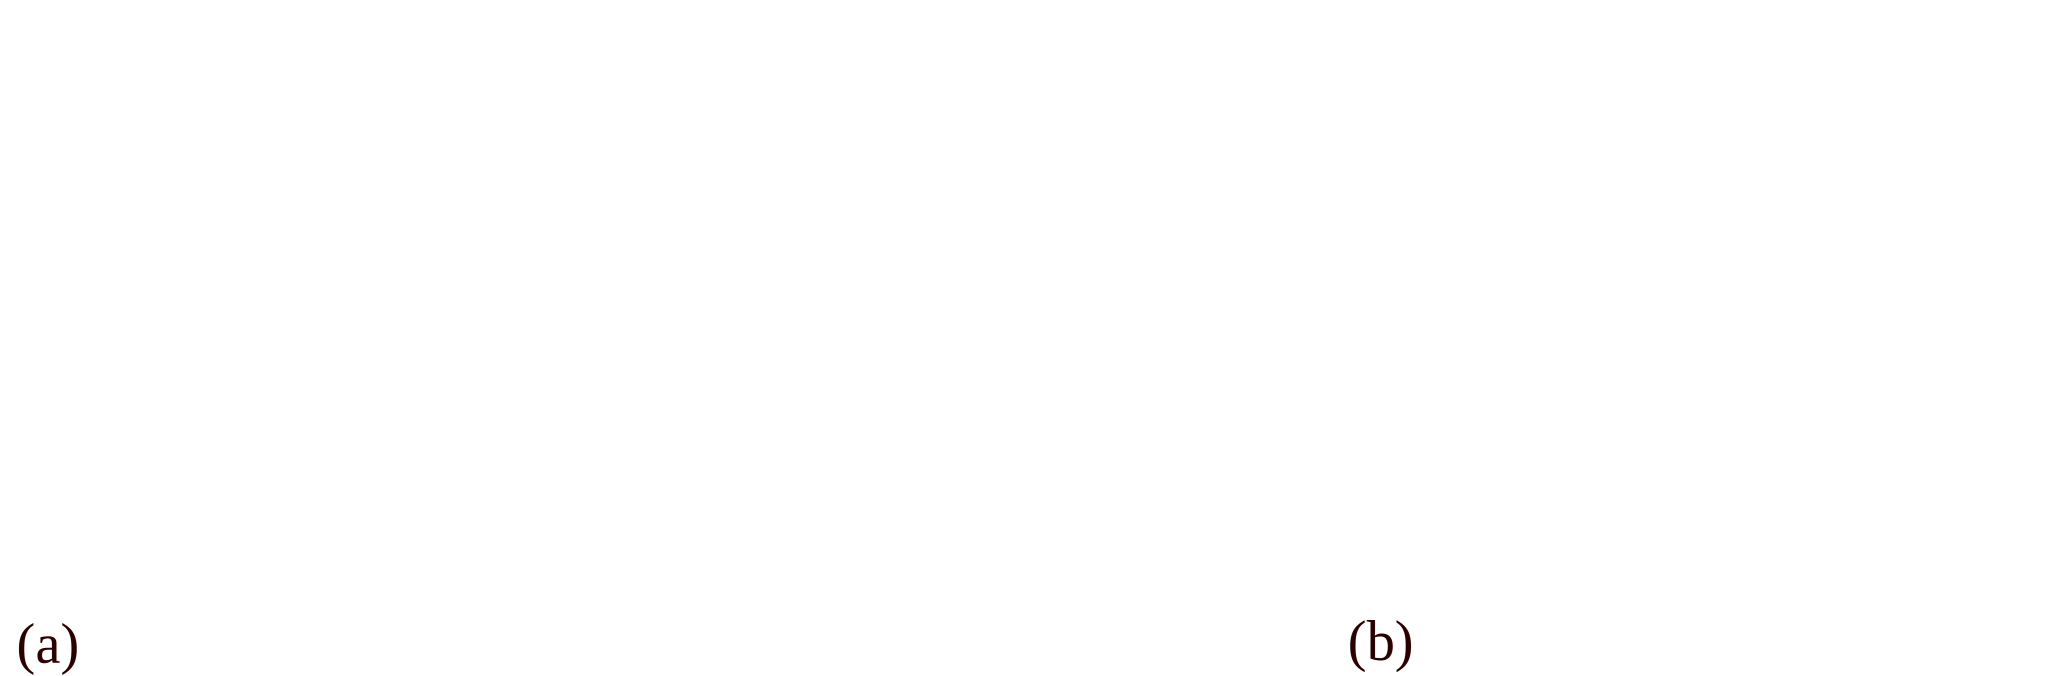
\includegraphics[width=0.8\linewidth]{./chapter04/Z2AZ2B.pdf}
	\caption{
		Visualization of the Z2A and Z2B \textit{Ans\"atze} with only nearest-neighbor couplings in (a) and (b), respectively. Blue and red colored bonds correspond to the prefactor +1 or -1, respectively, of the $U_{\bm{j}-\bm{i}}$ matrices specified by the corresponding \textit{Ansatz}.
	}
	\label{fig:chapter04_Z2AZ2B}
\end{figure}
%

Now, consider the so-called Z2B \textit{Ansatz}, which has the form~\cite{WenPLA2002}
%
\begin{equation}
	U_{\bm{i},\bm{j}} = (-1)^{(j_x-i_x) i_y} U_{\bm{j}-\bm{i}} \qquad {\rm and } \qquad A_0(\bm{i}) = 0,
\end{equation}
%
with $U_{\bm{j}-\bm{i}}$ defined as for the Z2A \textit{Ansatz} (see Figure~\ref{fig:chapter04_Z2AZ2B}~(b) for a visualization).
Translation in the $x$-direction transforms the \textit{Ansatz} as
%
\begin{align}
	\op{T}_x(U_{\bm{i},\bm{j}}) &= U_{\bm{i}-\uv{e}_x,\bm{j}-\uv{e}_x} \nonumber\\
								&= U_{\bm{i},\bm{j}}.
\end{align}
%
The corresponding gauge transformation $\op{G}_x$ is then seen to be specified by the uniform gauge transformation $G_x(i) = \tau^0$.
Translation in the $y$-direction, however, transforms the \textit{Ansatz} as
%
\begin{align}
	\op{T}_y(U_{\bm{i},\bm{j}}) &= U_{\bm{i}-\uv{e}_y,\bm{j}-\uv{e}_y} \nonumber\\
								&= (-1)^{(j_x-i_x)(i_y - 1)} U_{\bm{j}-\bm{i}} \nonumber\\
								&= (-1)^{i_x-j_x} U_{\bm{i},\bm{j}}.
\end{align}
%
Thus, the corresponding gauge transformation $\op{G}_y$ corresponds to the spatially-dependent gauge transformation $G_y(\bm{i}) = (-1)^{i_x} \tau^0$.
Note that the \textit{Ansatz} is \textit{not} invariant under translations in the $y$-direction, however, it is said to possess translation symmetry as it corresponds to a translationally invariant spin state due to the existence of the projective representation $\op{G}_y \op{T}_y$.
Additionally, the \textit{Ansatz} is seen to be invariant under global gauge transformations generated by $G_0(i) = -\tau^0$.
The projective symmetry group for the Z2B \textit{Ansatz} is then given by
%
\begin{equation}
	PSG_{\rm Z2B} = \avg{\{ \op{G}_0, \op{G}_x \op{T}_x, \op{G}_y \op{T}_y \}},
\end{equation}
%
where, to reiterate,
%
\begin{equation}
	G_0(i) = -\tau^0, \qquad G_x(i) = \tau^0, \qquad G_y(i) = (-1)^{i_x} \tau^0.
\end{equation}
%
The invariant gauge group is seen to be generated by the pure gauge transformations $\op{G}_0$, \ie,
%
\begin{equation}
	IGG_{\rm Z2B} =  \avg{\op{G}_0} \cong \ZZ.
\end{equation}
%

The \textit{Ans\"atze} Z2A and Z2B considered above are \textit{not} gauge equivalent.
Instead, they represent two \textit{distinct} \ZZ~spin liquid phases which possess all the same symmetries.
Whereas the paradigm of Landau's symmetry breaking is unable to distinguish between these two distinct quantum spin liquid phases, the projective symmetry group provides a way to probe their hidden order.
The implications of this quantum order for the low-energy excitations of the system have been glimpsed in Chapter~\ref{chapter:KitaevHoneycombModel} in the protection of Dirac fermions for the Kitaev honeycomb model.
These effects are explored further in the context of three-dimensional Kitaev spin liquids in Chapter~\ref{chapter:ClassificationOfKSL}.
As a warm-up, the following section will apply a modified form of the $SU(2)$ projective construction from Section~\ref{section:chapter04_ProjectiveConstructionOfQuantumSpinLiquids} to the Kitaev honeycomb model which has been adapted for application to Majorana fermions.


%
%%%%%%%%%%%%%%%%%%%%%%%%%%%%%%%%%%%%%%%%%%%%%%%%%%%%%%%%%%%%%%%%%%%%%%%%%%%%%%%%%%%%%%%%
\section{Application to the Kitaev honeycomb model}
\label{section:chapter04_ApplicationToTheKitaevHoneycombModel}
%%%%%%%%%%%%%%%%%%%%%%%%%%%%%%%%%%%%%%%%%%%%%%%%%%%%%%%%%%%%%%%%%%%%%%%%%%%%%%%%%%%%%%%%
%
The Kitaev honeycomb model presented in Chapter~\ref{chapter:KitaevHoneycombModel} is governed by the Hamiltonian
%
\begin{equation}
	\op{H} = -\sum_{\gamma{\rm -links}} J~\sigma^{\gamma}_j \sigma^{\gamma}_k, 
\end{equation}
%
where sites $j$ and $k$ are nearest-neighbors in the honeycomb lattice connected by a link of type $\gamma$ (refer to Chapter~\ref{chapter:KitaevHoneycombModel} for details) and the exchange couplings on all bonds have been chosen to be equal.
Substituting the spinon representation of Eq.~\eqref{eq:chapter04_SU2SpinonDefinition} into the Kitaev Hamiltonian yields the locally $SU(2)$ gauge invariant Hamiltonian
%
\begin{equation}
	\op{H} = -\frac{1}{4} \sum_{\gamma {\rm -links}} J~\trace{[F\dag_j \tau^{\gamma} F_j]} \trace{[F\dag_k \tau^{\gamma} F_k]}.
\end{equation}
%
A similar mean-field decoupling as was discussed in the previous sections for the Heisenberg model may be performed for the above Hamiltonian, however, the anisotropy of the Kitaev exchange makes for a significantly more cumbersome analysis~\cite{BurnellPRB2011}.
Instead, it has been pointed out~\cite{BurnellPRB2011,YouPRB2012,SeifertPRBFeb2018} that, given foreknowledge of the exact solution to the Kitaev model, it becomes much simpler to formulate the $SU(2)$ gauge theory in terms of Majorana fermions.

Introducing four Majorana operators at each site $c^{\gamma}$, where $\gamma = 0,x,y,z$ (the superscript for $c^0$ will be dropped for notational convenience and readability wherever it does not hinder clarity), defined in terms of the complex fermionic spinons as
%
\begin{equation}
	f_{j\uparrow} = \frac{1}{2} (c_j + ic^z_j) \qquad {\rm and } \qquad f_{j\downarrow} = \frac{1}{2} (ic^x_j - c^y_j),
\end{equation}
%
the $F$-matrices may be rewritten as
%
\begin{equation}
	F_j = \frac{1}{2} c_j^{\mu} T_{\mu},
\end{equation}
%
where $T = (\tau^0, i\tau^x, i\tau^y, i\tau^z)$.
The Majorana operators are normalized such that
%
\begin{equation}
\{c_j^{\mu}, c_k^{\nu}\} = 2\delta^{\mu\nu}\delta_{jk}.
\end{equation}
%
The spin-1/2 operators may now be expressed in terms of Majorana operators as
%
\begin{align}
	\sigma^{\gamma}_j &= \frac{1}{8} \trace{[c^{\mu}_j T\dag_{\mu} \tau^{\gamma} T_{\nu} c^{\nu}_j]} \nonumber\\
					  &= \frac{i}{4} c^{\mu}_j M^{\gamma}_{\mu\nu} c^{\nu}_j,
	\label{eq:chapter04_SpinMajoranaRepresentation}
\end{align}
%
where the three $4\times 4$ matrices
%
\begin{equation}
	M^{\gamma}_{\mu\nu} = -\frac{i}{2} \trace{[T\dag_{\mu} \tau^{\gamma} T_{\nu}]}
\end{equation}
%
form a representation of $\mathfrak{su}(2)$, \ie, $[M^{\alpha}, M^{\beta}] = 2\epsilon^{\alpha\beta\gamma} M^{\gamma}$.

For the half-filling constraint, one finds
%
\begin{equation}
	\frac{1}{2} \trace{[F_j \tau^{\gamma} F\dag_{j}]} = \frac{i}{4} c^{\mu}_j K^{\gamma}_{\mu\nu} c^{\nu}_j = 0,
	\label{eq:chapter04_HalfFillingConstraintMajorana}
\end{equation}
%
where the three $4\times 4$ matrices
%
\begin{equation}
	K^{\gamma}_{\mu\nu} = -\frac{i}{2} \trace{[T_{\mu} \tau^{\gamma} T\dag_{\nu}]}
\end{equation}
%
form another representation of $\mathfrak{su}(2)$ which, in fact, commutes with $M^{\gamma}$.
Thus, the local $SU(2)$ gauge-invariance of the Majorana representation in Eq.~\eqref{eq:chapter04_SpinMajoranaRepresentation} is seen to be generated by the matrices $K^{\gamma}$, \ie, gauge transformations take the form
%
\begin{equation}
	\bm{c}_j \rightarrow e^{\phi^{\mu}_j K^{\gamma}} \bm{c}_j,
\end{equation}
%
where $\bm{c}_j$ is the vector of Majorana operators at site $j$.
The half-filling constraint can be shown~\cite{SeifertPRBFeb2018} to reproduce the constraint $\op{D_j} = c_j c^x_j c^y_j c^z_j = 1$ for physical states as in Kitaev's original solution~\cite{KitaevAoP2006}.\footnote{The constraint here actually differs by a minus sign resulting from a choice of basis.}

With the above definitions, the Kitaev Hamiltonian may be written as a locally $SU(2)$ gauge-invariant Hamiltonian of interacting Majorana fermions
%
\begin{equation}
	\op{H} = -\frac{1}{16} \sum_{\avg{j,k}_{\gamma}} J \left(i\bm{c}\dag_j ~ M^{\gamma} ~ \bm{c}_j\right) \left(i\bm{c}\dag_k ~ M^{\gamma} ~ \bm{c}_k\right) - \frac{i}{4} \sum_j \bm{c}\dag_j ~ A_0(j) ~ \bm{c}_j,
\end{equation}
%
where $A_0(j) = \frac{1}{2} A^{\mu}_0(j) K^{\mu}$ is the temporal component of an $SU(2)$ gauge field enforcing the half-filling constraint of Eq.~\eqref{eq:chapter04_HalfFillingConstraintMajorana}.
Introducing the real Hubbard-Stratonovich matrix fields $U_{jk} = -U_{kj}$ to replace the Majorana bilinears $i c^{\mu}_j c^{\nu}_k$, the Kitaev Hamiltonian takes the form
%
\begin{equation}
	\op{H} = -\frac{J}{8} \sum_{\avg{j,k}_{\gamma}} \left(\frac{1}{2} \trace{[M^{\gamma} U_{ij} M^{\gamma} U_{ij}]} + i\bm{c}\dag_j ~ M^{\gamma} U_{ij} M^{\gamma} ~ \bm{c}_j\right) - \frac{i}{4} \sum_j \bm{c}\dag_j ~ A_0(j) ~ \bm{c}_j.
	\label{eq:chapter04_KitaevSU2}
\end{equation}
%
Hamiltonian~\eqref{eq:chapter04_KitaevSU2} is seen to describe a theory of Majorana fermions $\bm{c}_j$ coupled to a dynamic $SU(2)$ gauge field $(A_0(j), U_{jk})$, invariant under local $SU(2)$ gauge transformations $G_j = \exp{[\phi^{\mu}_j K^{\mu}]}$ as
%
\begin{align}
	\bm{c}_j	&\rightarrow G_j \bm{c}_j \nonumber\\
	A_0(j)		&\rightarrow G_j (A_0(j) + i \partial_t) G\dag_j \nonumber\\
	U_{jk}		&\rightarrow G_j U_{jk} G\dag_k.
\end{align}
%

At this stage, the zeroth order mean-field theory may be constructed by replacing the gauge field in Hamiltonian~\eqref{eq:chapter04_KitaevSU2} with a static mean-field \textit{Ansatz} $(i\ansatz{A}_0(j),~i\ansatz{U}_{jk})$ subject to the consistency conditions
%
\begin{equation}
	\ansatz{U}^{\mu\nu}_{jk} = \avg{i c^{\mu}_j c^{\nu}_k} \qquad {\rm and } \qquad \avg{\bm{c}\dag_j ~ \ansatz{A}_0(j) ~ \bm{c}_j} = 0.
\end{equation}
%
This mean-field theory may be solved to obtain the \textit{Ansatz}~\cite{YouPRB2012,SeifertPRBFeb2018}
%
\begin{equation}
	\begin{matrix*}[c]
		\ansatz{A}_0(j) 			= 0, \\
		\\
		\ansatz{U}^{\mu\nu}_{jk}	= \left\{
			\begin{matrix*}[l]
				-0.524866 &
				\qquad \text{for $\mu = \nu = 0$}\\
				1 &
				\qquad \text{for $\mu = \nu = \gamma$ and $(j,k) \in \avg{j,k}_{\gamma}$}\\
				0 &
				\qquad \text{otherwise,}
			\end{matrix*}
			\right.
	\end{matrix*}
\end{equation}
%
where a convention has been chosen such that site $j$ belongs to sublattice $A$ and site $k$ belongs to sublattice $B$.
For convenience of notation, let $u^{\mu}_{jk} = \ansatz{U}^{\mu\mu}_{jk}$, where no summation over repeated indices is implied.
Due to all $u^{\mu}_{jk}$ being unequal for any given link $\avg{j,k}$, the \textit{Ansatz} "breaks" the local $SU(2)$ gauge invariance down to a global \ZZ~gauge invariance, making the invariant gauge group \ZZ.
Note that, in agreement with the presentation of Chapter~\ref{chapter:KitaevHoneycombModel}, this mean-field \textit{Ansatz} implies the vanishing of spin-spin correlation functions beyond nearest neighbors with
%
\begin{equation}
	\avg{\sigma^{\alpha}_j \sigma^{\beta}_k} = - \delta_{\alpha\beta} \delta_{\avg{j,k}_\alpha} u^{\alpha}_{jk} u^0_{jk} = 0.524866.
\end{equation}
%

The zeroth order mean-field theory for the spin liquid may be written as
%
\begin{equation}
	\op{H} = -\frac{J}{8} \sum_{\avg{j,k}_{\gamma}} \left( i c_j u^{\gamma}_{jk} c_k + i c^{\gamma}_j u^0_{jk} c^{\gamma}_k \right) + {\rm const}.
	\label{eq:chapter04_KitaevZerothOrderMeanField}
\end{equation}
%
As a \ZZ~spin liquid, the fluctuations of the gauge field are known to be gapped and the first order mean-field theory is, thus, described by an identical Hamiltonian, albeit with the global \ZZ~gauge-invariance upgraded to a local invariance.
In fact, for the Kitaev spin liquid, the first order mean-field theory actually corresponds to the \textit{exact} solution where fluctuations of the gauge field are absent.
Diagonalization of Hamiltonian~\eqref{eq:chapter04_KitaevZerothOrderMeanField} yields three degenerate flat bands for $c^x, c^y$ and $c^z$ in addition to a graphene-like band structure for $c$ with Dirac nodes located at the $K$ and $K'$ points of the Brillouin zone~\cite{YouPRB2012,SeifertPRBFeb2018}.
The projective mean-field analysis is seen to reproduce Kitaev's original results presented in Chapter~\ref{chapter:KitaevHoneycombModel}.
With invariant gauge group $IGG = \ZZ$, the ground state of the Kitaev Hamiltonian corresponds to a stable, rigid spin liquid.

Having identified the low-energy \ZZ~theory for the Kitaev model, the projective symmetry group for the corresponding \textit{Ansatz} is considered.
The symmetry group for the Hamiltonian considered here will be $SG = \avg{\{ \op{T}_1, \op{T}_2, \op{\mathcal{P}}, \op{\mathcal{T}} \}}$, where $\op{T}_i$ generates translations along the $i^{\rm th}$ lattice vector $\ba_i$, $\op{\mathcal{P}}$ is the inversion operator and $\op{\mathcal{T}}$ is the time-reversal operator.
As varying the exchange couplings does not qualitatively affect the \textit{Ansatz} (in fact, it only changes the value of $u^0_{jk}$ for finite couplings) but \textit{does} break other lattice symmetries, \eg, rotation symmetry, these other symmetries will not be considered here.

Translation in the $\ba_1$-direction transforms the \textit{Ansatz} as
%
\begin{align}
	\op{T}_1 (i \ansatz{U}_{\bm{j}, \bm{k}})	&= i \ansatz{U}_{\bm{j}-\ba_1, \bm{k}-\ba_1} \nonumber\\
												&= i \ansatz{U}_{\bm{j}, \bm{k}}.
\end{align} 
%
The corresponding gauge transformation $\op{G}_{T_1}$ is then specified by the uniform gauge transformation $G_{T_1}(j) = \id$.
Similarly, one finds that the gauge transformation corresponding to translations in the $\ba_2$-direction is specified by the uniform gauge transformation $G_{T_2}(j) = \id$.

Inversion acts to map a bond of a given type into the same type of bond while simultaneously mapping sites from sublattice $A$ into sublattice $B$ and vice versa.
Taking advantage of translation symmetry, this action may be expressed simply as
%
\begin{align}
	\op{\mathcal{P}} (i \ansatz{U}_{\bm{j}, \bm{k}})	&= i \ansatz{U}_{\bm{k}, \bm{j}} \nonumber\\
														&= -i \ansatz{U}_{\bm{j}, \bm{k}}.
	\label{eq:chapter04_InversionOperation}
\end{align}
%
The associated gauge transformation $\op{G}_{\mathcal{P}}$ must act to cancel the minus sign in Eq.~\eqref{eq:chapter04_InversionOperation} and is seen to be specified by the spatially-dependent gauge transformation $G_{\mathcal{P}}(j) = (-1)^{\zeta_j} \id$, where
%
\begin{equation}
	\zeta_j = \left\{
		\begin{matrix*}[l]
			0 &
			\qquad \text{for $j \in$ sublattice $A$} \\
			&\\
			1 &
			\qquad \text{for $j \in$ sublattice $B$}.
		\end{matrix*}
	\right.
\end{equation}
%

The action of time-reversal on the \textit{Ansatz} is given by
%
\begin{equation}
	\op{\mathcal{T}} (i \ansatz{U}_{\bm{j}, \bm{k}}) = -i \ansatz{U}_{\bm{j}, \bm{k}}.
	\label{eq:chapter04_TimeReversalOperation}
\end{equation}
%
Similar to the inversion operation, the associated gauge transformation $\op{G}_{\mathcal{T}}$ must act to cancel the minus sign in Eq.~\eqref{eq:chapter04_TimeReversalOperation} and is seen to be specified by the spatially-dependent gauge transformation $G_{\mathcal{T}}(j) = (-1)^{\zeta_j} \id$, where $\zeta_j$ is defined as above.

The projective symmetry group for the Kitaev honeycomb model with symmetry group $SG$ is then given by
%
\begin{equation}
	PSG = \avg{\{ \op{G}_0, \op{G}_{T_1} \op{T}_1, \op{G}_{T_2} \op{T}_2, \op{G}_{\mathcal{P}} \op{\mathcal{P}}, \op{G}_{\mathcal{T}} \op{\mathcal{T}} \}},
\end{equation}
%
where $G_0(j) = -\id$ generates the invariant gauge group,
%
\begin{equation}
	G_{T_1}(j) = G_{T_2}(j) = \id \qquad {\rm and } \qquad G_{\mathcal{P}}(j) = G_{\mathcal{T}}(j) = (-1)^{\zeta_j} \id.
\end{equation}
%
As $\op{G}_\mathcal{P}$ and $\op{G}_{\mathcal{T}}$ are non-trivial, the \textit{Ansatz} is neither inversion- nor time-reversal invariant.
It is, however, both inversion and time-reversal \textit{symmetric} in the sense that it generates a physical spin state which possesses both symmetries.

Note that the gauge transformation $\op{G}_{\mathcal{T}}$ is simply a sublattice transformation.
Furthermore, as a combination of projective time-reversal and sublattice transformations, the action of $\op{\mathcal{T}}$ in the gauge-fixed sector actually corresponds to a particle-hole transformation $\op{\mathcal{C}}$ satisfying
%
\begin{equation}
	\{\op{\mathcal{C}}, \op{H}\} = 0.
	\label{eq:chapter04_ParticleHole}
\end{equation}
%
While not a property of the original spin Hamiltonian, the above relation is a property of the gauge-fixed Hamiltonian which holds true for Kitaev models with \textit{any} symmetry group.
It is merely a consequence of the Majorana representation.
Although the presence of particle-hole "symmetry" is, in this sense, trivial, the restriction it poses to the fermionic quasiparticle spectrum will be seen in the following chapter to play an important role for the low energy properties of the system.


%
%
%%%%%%%%%%%%%%%%%%%%%%%%%%%%%%%%%%%%%%%%%%%%%%%%%%%%%%%%%%%%%%%%%%%%%%%%%%%%%%%%%%%%%%%%
\section{Summary}
\label{section:chapter04_Summary}
%%%%%%%%%%%%%%%%%%%%%%%%%%%%%%%%%%%%%%%%%%%%%%%%%%%%%%%%%%%%%%%%%%%%%%%%%%%%%%%%%%%%%%%%
%
%
This chapter introduced the concept of \textit{quantum order}, an idea proposed to characterize the phases of matter to which Landau's theory of phase transitions and classical order cannot be applied.
Such phases of matter are not characterized by the spontaneous breaking of a continuous symmetry and the ideas of long-range order and local order parameters of Landau's theory are rendered inoperative.
Instead, the description of such phases requires the development of new theoretical tools.

The focus of this chapter was on one such tool called the \textit{projective symmetry group}.
The projective symmetry group was introduced in the context of classifying different quantum spin liquids with the same symmetries.
By employing a fermionic representation of spins, a spin-1/2 model may be rewritten as a fermionic model with a local $SU(2)$ gauge redundancy and analyzed using a mean-field gauge \textit{Ansatz}.
The stability of such a mean-field spin liquid depends in part upon the leftover -- and potentially reduced -- gauge redundancy of the \textit{Ansatz} which defines the so-called \textit{invariant gauge group}.
When represented in the fixed gauge sector of the mean-field spin liquid, physical symmetries must be supplemented by a gauge transformation from the invariant gauge group.
The set of all such symmetry operations acting on the mean-field spin liquid forms the projective symmetry group.
In this way, spin liquids with the same physical symmetry group are seen to possess different \textit{projective} symmetry groups and, thus, correspond to distinct spin liquid phases with different quantum order.

After a detailed discussion of these ideas, the machinery of the projective symmetry group was applied to the Kitaev honeycomb model introduced in Chapter~\ref{chapter:KitaevHoneycombModel}.
Here it was seen that the projective symmetry group is responsible for the stability of the gapless Dirac fermions in the Kitaev spin liquid.
In the next chapter, these ideas will be used to show how Kitaev spin liquids on different three-dimensional lattices may host a variety of gapless excitations, the existence of which are enforced by their unique projective symmetry groups.